\documentclass[assignment02_Solutions]{subfiles}

\invalidatemargin

\IfSubStr{\jobname}{\detokenize{Solutions}}{\toggletrue{solutions}}{\togglefalse{solutions}}

\fancypagestyle{firstpage}

{\rhead{Assignment 2 \linebreak \textit{Version: \today}}}

\title{Assignment 2: (Un)Fairness and Probability}
\author{Machine Learning}
\date{Fall 2019}

\renewcommand{\arraystretch}{3}
\begin{document}

\maketitle
\thispagestyle{firstpage}


\begin{learningobjectives}
\bi
\item The concept of independence and conditional independence
\item The basic components of a Bayesian Networks (BN)
\item The rules of d-separation to compute conditional independence relationships in a BN
\item The Compas recidivism risk algorithm controversy
\ei
\end{learningobjectives}

Note: This assignment is a bit longer than average. We are trying to shift things so that weekend assignments are a bit longer and the assignments during the week are a bit shorter. If you decide to ask for an extension, we suggest that you prioritize looking at the COMPAS Model section, so that you are prepared for our class discussion.

A quick thanks to two former students, Micah Reid (currently a CA) and Miranda Lao for their contributions to this and the following assignment. As part of their final project, they explored metrics of fairness and disparity and proposed assignment extensions (pieces of which appear in this and the following assignment). 

\section{COMPAS Model: Race, Criminal Justice, and Machine Learning}

\begin{notice}
We are going to think about race and criminal justice in the United States. Before we dive into this, we want to acknowledge:

\bi
\item This is a complex and intricate issue that involves policy, society, technology, individual beliefs/values, and history. This topic directly (but not equally) impacts the lives of many people.
\item We all have our own lenses through which we view the world.
\item In this class, we will scratch the surface of the way the US justice system works. Your instructors are not criminal justice experts, but they do care about this topic. We are also continuing to learn more.
\item This topic will likely be uncomfortable to grapple with regardless of your background and identity. It may resonate differently with each of us. We (Sam/Carrie) are available in person and via email, if you would like to discuss how we can best support you in class. We are planning to have some group discussion in class. One method of support could be pairing you with a partner of your choosing for this discussion. Another could be including your ideas about how class discussion can be informative and challenging without creating unnecessary pain. Please reach out to us if you have any concerns or want to discuss this more.
\ei
\end{notice}

A few basics about the US criminal criminal justice system. 

A police officer can place a person under arrest. However, an arrest does not necessarily mean that person committed a crime (both in fact and in a legal sense). Legally, someone is considered innocent until proven guilty in court. However, arrested people are often held in jail for months before trail (this is called pretrial detention). To get out of jail before trial, the arrested person can post bail. Bail is a considerable amount of money (``money bond'') that is given to the court to ensure the person shows up to trial. As you might guess, bail represents a way people with money are treated differently by the system than people without money.  (Optional: For more on bail, listen to \href{https://www.earhustlesq.com/episodes/2021/9/22/do-it-movin}{Episode 62} of the podcast Ear Hustle). 

Legally, a person is considered guilty if they are convicted in court. Practically, innocent people are sometimes convicted. People with a lot of money can hire many lawyers who will work many days, weeks, or years, fighting the case. People without funds for a lawyer will be assigned a public defender. Public defenders are often overwhelmed, and might have just a minute to look over the details of a case, right before trail.

If you are interested in this topic and want to hear stories from incarcerated people, we recommend listening to the podcast \href{https://www.earhustlesq.com/}{Ear Hustle}. (This is optional) 


\begin{exercise}[\faShareAlt~(20 minutes)]
\bes
\item (Read the Report of \href{https://www.sentencingproject.org/publications/un-report-on-racial-disparities/}{The Sentencing Project to the United Nations Special Rapporteur on Contemporary Forms of Racism, Racial Discrimination, Xenophobia, and Related Intolerance}. 

This article is intended to provide some background information on criminal justice and race in the US. 
\ees
\end{exercise}



\subsection{Confusion Matrices}
Before we dig into the articles on the COMPAS algorithm, we want to introduce \/ refresh on the confusion matrix and some related terms. These will be essential to making sense of the debate below and for learning about different metrics of fairness. The binary confusion matrix is a 2x2 chart where the y axis is whether the model output predicts a positive or negative response, and the x axis is whether or not the actual or measured output is positive or negative. This gives us four quadrants: true positives, false positives, true negatives, and false negatives.\\

\begin{center}
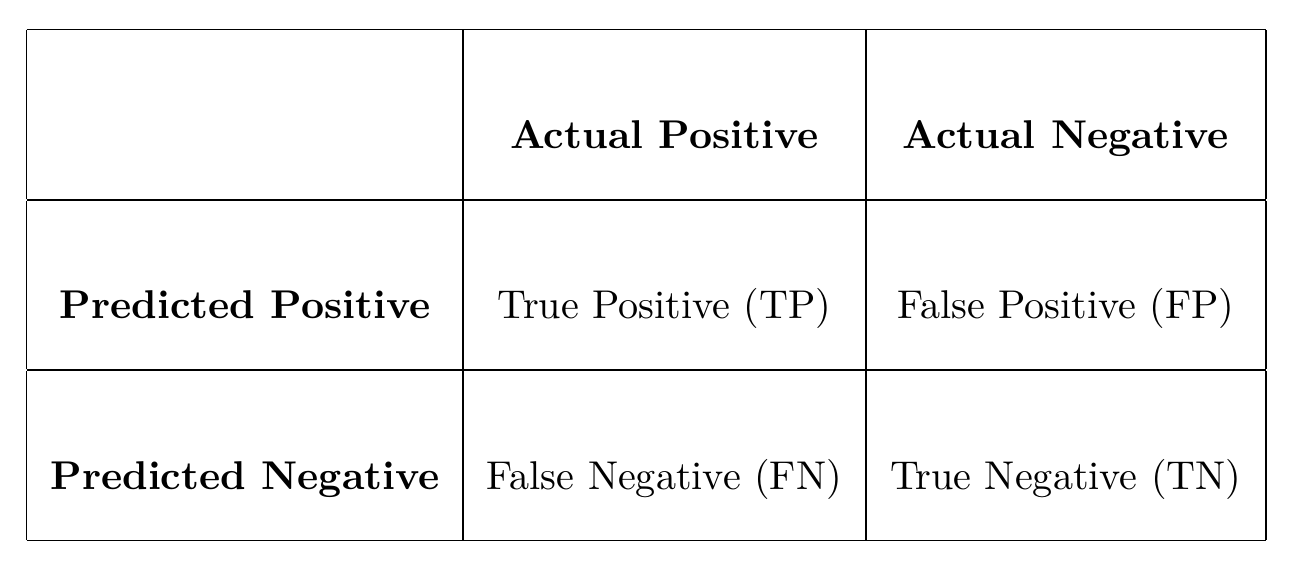
\includegraphics[width=0.5\linewidth]{figures/confusion}
\end{center}
%\begin{center}
%\begin{tabular}{|m|m|m|} 
%\hline
%& \textbf{Actual Positive} & \textbf{Actual Negative} 
%\hline
%\textbf{Predicted Positive} & True Positive (TP) & False Positive (FP) 
%\hline
%\textbf{Predicted Negative} & False Negative (FN) & True Negative (TN) \\ 
%\hline
%\end{tabular}
%\end{center}

It is worth stating that the confusion matrix only works for classification, so if the model outputs are continuous, a cutoff threshold may be necessary. These confusion matrix metrics can be more informative than more general accuracy metrics like log loss, because they can pinpoint the strong and weak points of a model. The four quadrants can also be used to calculate a number of metrics that can show how the model performs with regards to different concerns. \\

These definitions are relatively straightforward. We call the total number of actual positives the \textbf{condition positive (P)}, where $P = TP + FN$. The total number of actual negatives is the \textbf{condition negative (N)}, where $N = FP + TN$. \\

A variety of combinations of these 4 quadrants (TP, FP, FN, and TN) are found in the building blocks widely used fairness metrics in machine learning. These building blocks include:

\bi
\item \textbf{True Positive Rate (TPR): } $TPR = \frac{TP}{P}$
\item \textbf{True Negative Rate (TNR): }  $TNR = \frac{TN}{N}$
\item \textbf{False Positive Rate (FPR): } $FPR = \frac{FP}{P}$
\item \textbf{False Negative Rate (FNR): } $FNR = \frac{FN}{P}$
\item \textbf{Positive Predictive Value (PPV): } $PPV = \frac{TP}{TP+FP}$
\item \textbf{Negative Predictive Value (NPV): } $NPV = \frac{TN}{TN+FN}$
\item \textbf{False Discovery Rate (FDR): } $FDR = \frac{FP}{TP+FP}$
\item \textbf{False Omission Rate (FOR): } $FOR = \frac{FN}{TN+FN}$
\ei

It may be helpful to check out this \href{https://research.google.com/bigpicture/attacking-discrimination-in-ml/}{write-up from Google of the loan example}. The visualizations are good.

\begin{exercise}[\faShareAlt~(30 minutes)]
Consider the following confusion matrix:
\begin{center}
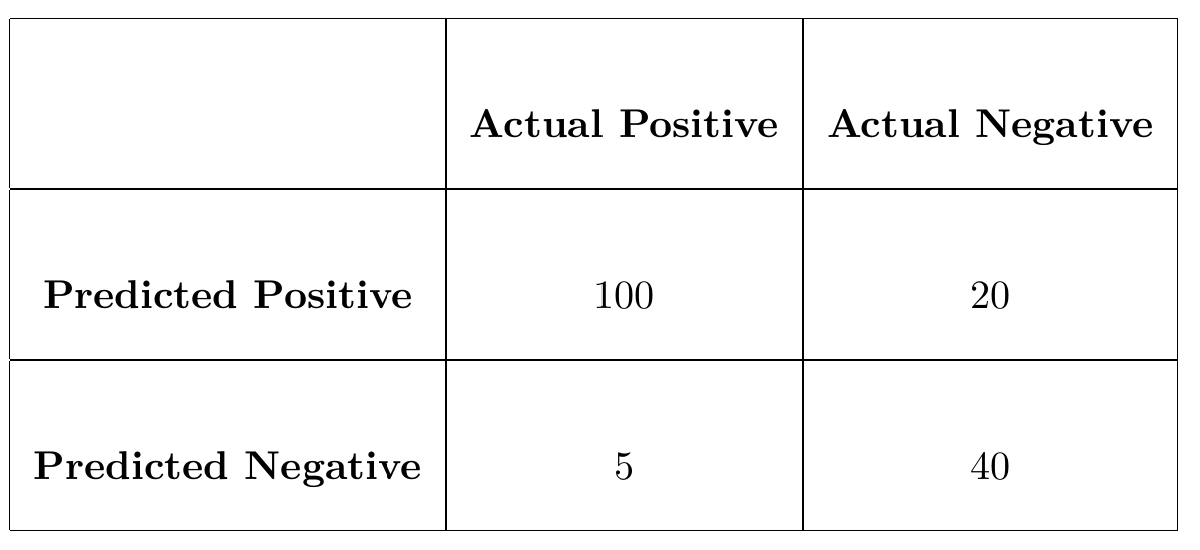
\includegraphics[width=0.5\linewidth]{figures/confusionNumbers}
\end{center}

\bes
\item Compute the metrics listed above for this confusion matrix. \\

\begin{boxedsolution}
$\textbf{TPR =} 100 / (100 + 5) \approx .95$\\
$\textbf{FPR =} 20  / (20 + 40) \approx .33$\\
$\textbf{PPV =} 100 / (100 + 20) \approx .83$\\
$\textbf{NPV =} 40 / (40 + 5) \approx .89$\\
$\textbf{TNR =} 40 / (40 + 20) \approx .67$\\
$\textbf{FNR =} 5 / (100 + 5) \approx .05$\\
$\textbf{FDR =} 20 / (100 + 20) \approx .17$\\
$\textbf{FOR =} 5 / (5 + 40) \approx .11$\\
$\textbf{CSI =} 100 / (100 + 5 + 20) = .8$
\end{boxedsolution}

\item If you've completed part a, you may have noticed that each metric above other than CSI has an inverse (for example the True Positive Rate is equal to 1 - False Negative Rate). Find the inverse for each of the metrics listed above.


\begin{boxedsolution}
True Positive Rate is the inverse of False Negative Rate.\\
True Negative Rate is the inverse of False Positive Rate.\\
Positive Predictive Value is the inverse of False Discovery Rate.\\
Negative Predictive Value is the inverse of False Omission Rate.\\
\end{boxedsolution}

\i

\item Consider the following scenarios: imagine you are creating a model to determine whether someone should be brought in for an additional cancer screening based upon initial test results. Which metric would you care most about minimizing? What if instead you were creating a model to determine whether a defendant should be prosecuted for a low level offense?

\begin{boxedsolution}
This depends on your own philosophy and strategy. We will explore some general guidance on this later.
\end{boxedsolution}
\ees

\end{exercise}

\begin{exercise}[\faShareAlt~(90 minutes)]
In this module, we'll be spending time talking about the Correctional Offender Management Profiling for Alternative Sanctions (COMPAS) algorithm, produced by the company Northpointe, Inc. COMPAS was intended to assess the risk of recidivism. This is a well-known algorithm in machine learning communities. 

Below we will provide you a list of readings on this topic. As you read, please prepare to reflect on the following themes:
\bi
\item Social justice in a non-ideal world.
\item The roles of machine learning engineers and the roles of other professional roles in the application of machine learning in our society.
\item The major things that you would want to consider in this type of undertaking.
\item Framing things mathematically versus from a social justice standpoint.
\item The level of technical debate in model choices that is brought up in this discussion (especially in the technical responses). 
\ei

\bes
\item First, read the \href{https://www.propublica.org/article/machine-bias-risk-assessments-in-criminal-sentencing}{ProPublica article.}

\item Next, you'll read the technical details of the ProPublica analysis.

We would like to be clear about when the COMPAS metric is applied. It is applied after someone is arrested, and the prediction COMPAS gives is if that person will be arrested again. A person who was arrested twice could be legally and actually innocent. It is important to be clear in our language that these are arrested people, and not convicted criminals. The term recidivism, which is generally defined as a criminal who commits a second crime, is used in the readings. ProPublica actually redefines recidivism as ``a criminal offense that resulted in a jail booking and took place after the crime for which the person was COMPAS scored.'' Here, ProPublica conflates an arrest for a crime with a conviction for that crime. Note that a jail booking is pre-trial, and different than prison, which is post-trial and conviction. This language is also used by the Northpointe rebuttal. Carrie would argue that since these are not people who have been yet convicted of crimes, they are not necessarily recidivists, and the language in the readings should be corrected.

Please read \href{https://www.propublica.org/article/how-we-analyzed-the-compas-recidivism-algorithm}{How We Analyzed the COMPAS Recidivism Algorithm.}

\item Please read the \href{https://drive.google.com/file/d/1SSbotzlsVkj4L2VhPC7R_XH0VBqOQsnT/view?usp=sharing}{Northpointe rebuttal}. This is a long reading. It has a lot of jargon, and some acronyms are not defined. We strongly suggest limiting yourself to 60 minutes for this reading (perhaps read the conclusion early on). You may consider working with a classmate on this reading, so you can both discuss what you think the author is saying. We're including this whole reading here because we would like you to engage with the real-world material.
\ees
\end{exercise}

\begin{exercise}[\faShareAlt~(40 minutes)]
\bes
%\item (10 minutes for this part) \href{http://nb.mit.edu/f/56089}{Read the Injustice Ex Machina: Predictive Algorithms in Criminal Sentencing} for a high-level perspective.
\item Please summarize what you see as the key parts of the ProPublica and Northpointe cases. You can use words, diagrams, concept maps, or another method that works for you.
\item Reflect on what you've just read.  We think the themes brought up above will provide good fodder for your response, but please feel free to take it in any direction.  Aim for around two paragraphs in your response.
\ees
\end{exercise}





\section{Motivation and Context for Probability}
In the last assignment we learned the basic definition of a probability and acquired some very powerful rules for working with probabilities.  In the rest of this assignment you'll be taking these ideas and extending them in the following significant ways.

\bi
\item You'll learn a graphical way to represent the relationships between probabilities that will make it much easier to work with large probabilistic models.
\item You'll be taking the ideas of probability using them to derive a whole new way of approaching the classification problem in machine learning.
\ei


\section{Product Rule and Marginalization for Random Variables}
\begin{recall}[Product Rule and Marginalization for Events]
Last assignment we learned about two very powerful techniques for computing the probability of events.
\bi
\item We learned the product rule (or conjunction rule), which states that for any two events $\mathcal{A}$ and $\mathcal{B}$,
\begin{align}
p(\mathcal{A}, \mathcal{B}) &= p(\mathcal{A}) p(\mathcal{B}|\mathcal{A}) \label{eq:prodcutruleevents} \\
&= p(\mathcal{B}) p(\mathcal{A}|\mathcal{B}) \enspace  . \nonumber
\end{align}
\item We learned the rule of marginalization, which states that for any two events $\mathcal{A}$ and $\mathcal{B}$,
\begin{align}
p(\mathcal{A}) &= p(\mathcal{A}, \mathcal{B}) + p(\mathcal{A}, \neg \mathcal{B}) \label{eq:marginalizationevents} \enspace .
\end{align}
\ei
It turns out that these rules can modified slightly to apply to random variables as well (instead of just events).
\end{recall}


\subsection{Product Rule for Random Variables}
Suppose we have two random variables $X$ and $Y$.  If we want to know the probability of random variable $X$ taking on value $x$ (it is common to use a lower case letter to refer to a particular value of a random variable) and random variable $Y$ simultaneously taking on value $y$, we can decompose the joint probability (the probability of both of these things occurring simultaneously) using the product rule.

\begin{align}
p(X = x, Y = y) &= p(X=x)p(Y=y | X=x) & \mbox{or equivalently,}\\
&= p(Y=y)p(X=x|Y=y) \nonumber
\end{align}

Notice that this looks pretty much identical to Equation~\ref{eq:prodcutruleevents} except that instead of referencing whether an event happens, we are now referencing a random variable taking on a particular value.

\begin{notice}
It's very common to use the shorthand $p(x, y)$ to refer to $p(X = x, Y = y)$.  The motivation for this shorthand is that it is obvious from the context that $p(x, y)$ really means the probability of random variable $X$ taking on value $x$ and random variable $Y$ taking on value $y$.  In this assignment we're going to avoid using this shorthand, but we will start using the shorthand in future assignments (we'll warn you when we start using it).  Also, you may see this notation used in external resources, so it helps to know about it.
\end{notice}

\subsection{Marginalization for Random Variables}
Again, suppose we have two random variables $X$ and $Y$.  We are interested in computing $p(X = x)$, but suppose it is difficult to compute this probability directly.  Just as we did for events in the last assignment, we can compute $p(X=x)$ by marginalizing out the random variable $Y$.  For simplicity, let's assume that $Y$ can only take on integer values from 1 to $k$.  We can write the marginal distribution $p(X=x)$ in the following way.

\begin{align}
p(X=x) &= \sum_{y=1}^k p(X=x, Y=y)\label{eq:rvmarginal}
\end{align}

You should notice that this equation is similar to Equation~\ref{eq:marginalizationevents} except that instead of summing over the probability for the two possible outcomes with respect to the event $\mathcal{B}$ (i.e., $\mathcal{B}$ either happens or it does not), we are now summing over the $k$ possible values that $Y$ could take.  Random variables don't necessarily have to take on values from 1 to $k$.  In general, if the random variable $Y$ can take on any value from some discrete set of values $\mathcal{Y}$ (we are using the calligraphic font because we are referring to a set), then the marginal distribution of $X$ can be written as:
\begin{align}
p(X=x) &= \sum_{y \in \mathcal{Y}} p(X=x, Y=y) \enspace . \label{eq:rvmarginalgeneral}
\end{align}
Notice that Equation~\ref{eq:rvmarginal} is a special case of Equation~\ref{eq:rvmarginalgeneral} where $\mathcal{Y} = \{1, 2, \ldots, k\}$.

\begin{exercise}[(15 minutes)]
This exercise is from the \href{https://en.wikipedia.org/wiki/Marginal_distribution\#Real-world_example}{Wikipedia article on marginal distribution}.

\vspace{1em}

\begin{notice}
Strictly speaking a random variable only takes on real numbers as its value (i.e., a random variable cannot take on the value of ``blue'').  That said, it's common to see folks bend this rule a bit by allowing the random variable to take on values that are not real numbers (e.g., you will see that in the Wikipedia article linked above).  Allowing for random variables to have non-numeric values doesn't really change the math except it makes it meaningless to compute quantities such as the mean.  Since in many cases allowing random variables to take on non-numeric values will make things clearer, we will allow this in our materials.
\end{notice} 
\vspace{1em}

Suppose you want to compute the probability that a pedestrian will be hit by a car, while crossing the road at a pedestrian crossing, without paying attention to the traffic light (a bit morbid, we know).  Let $H$ be a discrete random variable taking on the value ``$\mbox{hit}$'' if the pedestrian is struck and ``$\mbox{not hit}$'' if the pedestrian makes it safely across.  Let $L$ (for traffic light) be a discrete random variable taking on the value ``$\mbox{red}$'' when the light is red, ``$\mbox{yellow}$'' when the light is yellow, and ``$\mbox{green}$'' when the light is green.

The model that governs the prior probability of the light ($L$) is as follows.
\begin{align}
p(L = \mbox{red}) = 0.2 \nonumber \\
p(L = \mbox{yellow}) = 0.1 \nonumber \\
p(L = \mbox{green}) = 0.7
\end{align}
The model that governs the conditional probability of $H$ given $L$ is as follows.
\begin{align}
p(H = \mbox{hit} | L = \mbox{red}) = 0.01 \nonumber \\
p(H = \mbox{not hit} | L = \mbox{red}) = 0.99 &~~~~\mbox{Note: the probability of ``not hit''  = 1 - probability of hit} \nonumber \\
p(H = \mbox{hit} | L = \mbox{yellow}) = 0.1 \nonumber \\
p(H = \mbox{not hit} | L = \mbox{yellow}) = 0.9 \nonumber \\
p(H = \mbox{hit} | L = \mbox{green}) = 0.8  \nonumber \\
p(H = \mbox{not hit} | L = \mbox{green}) = 0.2 \nonumber
\end{align}

What is $p(H=\mbox{hit})$?

\begin{boxedsolution}
\begin{align}
p(H = \mbox{hit}) &= p(H = \mbox{hit}, L = \mbox{red}) +  p(H = \mbox{hit}, L = \mbox{yellow}) +  p(H = \mbox{hit}, L = \mbox{green}) &\mbox{marginalization} \nonumber \\
&= p(L = \mbox{red}) p(H = \mbox{hit} | L = \mbox{red}) + p(L = \mbox{yellow}) p(H = \mbox{hit} | L = \mbox{yellow}) &\mbox{product rule}\nonumber \\
&\hspace{0.5in}+ p(L = \mbox{green}) p(H = \mbox{hit} | L = \mbox{green}) \nonumber\\
&= (0.2 \times 0.01) + (0.1 \times 0.1) + (0.7 \times 0.8) \nonumber \\
&= 0.572 \nonumber
\end{align}
\end{boxedsolution}
\end{exercise}

\section{Some Twists on Bayes' Rule}

By now hopefully you are starting to feel comfortable with the vanilla form of Bayes' rule.  There are a few quite useful variants that we'd like to point out.  There are no exercises for you to do here, just add these to your bag of tricks (you'll be leveraging them later in this assignment, so you'll have a chance to solidify them then).

\begin{align}
p(\mathcal{A} | \mathcal{B}) &= \frac{p(\mathcal{B}|\mathcal{A}) p(\mathcal{A})}{p(\mathcal{B})} & \mbox{as a reminder, here is vanilla Bayes' rule} \\
p(\mathcal{A}, \mathcal{B} | \mathcal{C}) &= \frac{p(\mathcal{C}|\mathcal{A}, \mathcal{B}) p(\mathcal{A, B})}{p(\mathcal{C})} & \mbox{you can bring over multiple events} \\
p(\mathcal{A} | \mathcal{B}, \mathcal{C}) &= \frac{p(\mathcal{B} | \mathcal{A}, \mathcal{C}) p(\mathcal{A}|\mathcal{C})}{p(\mathcal{B}|\mathcal{C})} & \mbox{you can leave an event to the right of the conditioning bar}
\end{align}

\section{Independence and Conditional Independence}

Two of the most important concepts in probability theory are independence and the closely related concept of conditional independence.  These ideas are important because they let you analyze probabilistic quantities in isolation.  For instance, if you know that two events that you are interested in predicting are independent of each other, then you can make a model of each event in isolation.  Modeling events independently can make your life much easier since you don't have to consider how the two events interact.  Next, we'll make this high-level idea precise.

\subsection{Independence}
The product rule of probability can be simplified when two events, $\mathcal{A}$ and $\mathcal{B}$ are independent.  As an example, suppose $\mathcal{A}$ represents the event that the first flip of a coin comes up heads and event $\mathcal{B}$ is the event that the second flip of the same coin comes up heads.  Since whether or not $\mathcal{A}$ occurs tells us nothing about whether $\mathcal{B}$ would occur, we say that $\mathcal{A}$ and $\mathcal{B}$ are independent events (we use the notation $\mathcal{A} \condindep \mathcal{B}$ to indicate that $\mathcal{A}$ is independent of $\mathcal{B}$).  An event $\mathcal{A}$ is independent of another event $\mathcal{B}$ if and only if the following condition holds.
\begin{align}
p(\mathcal{A}, \mathcal{B}) &= p(\mathcal{A}) p(\mathcal{B}) \label{eq:indepevents}
\end{align}

A direct consequence of Equation~\ref{eq:indepevents} is that if $\mathcal{A} \condindep \mathcal{B}$, then
\begin{align}
p(\mathcal{A} | \mathcal{B}) &= p(\mathcal{A}) & \mbox{and} \nonumber \\
p(\mathcal{B} | \mathcal{A}) &= p(\mathcal{B}) \enspace . \nonumber
\end{align}

A very similar equation to Equation~\ref{eq:indepevents} can be defined for random variables.  Two random variables $X$ and $Y$ are independent if and only if the following condition holds for any values $x$ and $y$.

\begin{align}
p(X=x, Y=y) &= P(X=x) p(Y=y)
\end{align}
Similar to the rule for events, $p(X=x | Y=y) = P(X=x)$ if $X \condindep Y$.

\begin{exercise}[(10 minutes)]
\bes
\item Provide at least 3 examples of events or random variables that are independent of each other.

\begin{boxedsolution}
\bi
\item The event that a coin comes up heads on the first throw and the event that the coin comes up heads on the second throw.
\item A random variable that represents that last digit on a car's license plate and a random variable that represents the last digit on another car's license plate.
\item The event that captures whether or not it rains tomorrow in Boston and a random variable that represents the number of people who attend a rock concert in California tomorrow night (at least it seems that these things are unrelated).
\ei
\end{boxedsolution}

\item Provide at least 3 examples of events or random variables that are not independent of each other.

\begin{boxedsolution}
Here are some ideas.
\bi
\item The daily increase in the Dow Jones Industrial average and the daily increase in the NASDAQ.
\item The event that the American League wins the World Series in 2019 and the event that the National League wins the World Series in 2019.
\item The probability that it's raining today and the probability that it will rain tomorrow.
\ei
\end{boxedsolution}

\ees
\end{exercise}

\subsection{Conditional Independence}
Sometimes two events (or two random variables) that are not independent might become independent when conditioned on another event.

\begin{exercise}[(20 minutes)]

As a motivating example for the concept of conditional independence, consider a variant of the coin problem we saw last assignment.  A bag contains two coins.  Suppose we choose one of the two coins with equal probability.  Let $\mathcal{C}_1$ represents the event that we choose coin 1 and $\mathcal{C}_2$ represent the event that we choose coin 2.  Coin 1 is fair $p(\mathcal{H} | \mathcal{C}_1) = \frac{1}{2}$.  Coin 2 is not fair ($p(\mathcal{H} | \mathcal{C}_2) = \frac{4}{5}$).   We then flip the coin twice (we don't pick a new coin for the second flip).  Let $\mathcal{H}_1$ represent the event that the first flip comes up heads and $\mathcal{H}_2$ represent the event that the second flip comes up heads.  Are $\mathcal{H}_1$ and $\mathcal{H}_2$ independent (i.e., is $\mathcal{H}_1 \condindep \mathcal{H}_2$)?

To help you get started, here is a tree diagram illustrating the problem.

\begin{center}
\includegraphics[width=\linewidth]{figures/twocoins}
\end{center}
Given the tree diagram above, is $\mathcal{H}_1 \condindep \mathcal{H}_2$?

\begin{boxedsolution}

In order to test $\mathcal{H}_1 \condindep \mathcal{H}_2$ we need to check the following condition:
\begin{align}
p(\mathcal{H}_1, \mathcal{H}_2) \stackrel{?}{=} p(\mathcal{H}_1) p(\mathcal{H}_2)
\end{align}

We can compute each of the terms in the preceding equation using the tree diagram.  In total there are 8 possible paths through the tree.  Recall that we can find the probability of a path by multiplying the numbers on the lines.  To find the probability of a particular event, say $p(\mathcal{H}_1)$ we just add up the probability of all of the paths that include $\mathcal{H}_1$.  We can apply this technique to each of the events we care about.

\begin{align}
p(\mathcal{H}_1) &= p(\mathcal{C}_1, \mathcal{H}_1, \mathcal{H}_2) +  p(\mathcal{C}_1, \mathcal{H}_1, \neg \mathcal{H}_2)+  p(\mathcal{C}_2, \mathcal{H}_1, \mathcal{H}_2) +  p(\mathcal{C}_2, \mathcal{H}_1, \neg \mathcal{H}_2) \nonumber \\
&= \left ( \frac{1}{2} \times \frac{1}{2} \times \frac{1}{2}  \right) + \left ( \frac{1}{2} \times \frac{1}{2} \times \frac{1}{2} \right ) + \left ( \frac{1}{2} \times \frac{4}{5} \times \frac{4}{5}  \right) + \left ( \frac{1}{2} \times \frac{4}{5} \times \frac{1}{5} \right )\nonumber \\
&= \frac{13}{20} \nonumber \\
p(\mathcal{H}_2) &= p(\mathcal{C}_1, \mathcal{H}_1, \mathcal{H}_2) +  p(\mathcal{C}_1, \neg \mathcal{H}_1, \mathcal{H}_2)+  p(\mathcal{C}_2, \mathcal{H}_1, \mathcal{H}_2) +  p(\mathcal{C}_2, \neg \mathcal{H}_1, \mathcal{H}_2) \nonumber \\
&= \left ( \frac{1}{2} \times \frac{1}{2} \times \frac{1}{2}  \right) + \left ( \frac{1}{2} \times \frac{1}{2} \times \frac{1}{2} \right ) + \left ( \frac{1}{2} \times \frac{4}{5} \times \frac{4}{5}  \right) + \left ( \frac{1}{2} \times \frac{1}{5} \times \frac{4}{5} \right )\nonumber \\
&= \frac{13}{20} \nonumber \\
p(\mathcal{H}_1, \mathcal{H}_2) &=  p(\mathcal{C}_1, \mathcal{H}_1, \mathcal{H}_2) + p(\mathcal{C}_2, \mathcal{H}_1, \mathcal{H}_2) \nonumber \\
&= \left ( \frac{1}{2} \times \frac{1}{2} \times \frac{1}{2} \right ) + \left ( \frac{1}{2} \times \frac{4}{5} \times \frac{4}{5} \right ) \nonumber \\
&= \frac{89}{200} \nonumber \\
p(\mathcal{H}_1) p(\mathcal{H}_2) &= \frac{13}{20} \times \frac{13}{20} = \frac{169}{400} \neq \frac{89}{200} = p(\mathcal{H}_1, \mathcal{H}_2) \nonumber
\end{align}
Since $p(\mathcal{H}_1, \mathcal{H}_2) \neq p(\mathcal{H}_1) p(\mathcal{H}_2)$, $\mathcal{H}_1$ is not independent of $\mathcal{H}_2$.

\end{boxedsolution}
\end{exercise}

It turns out that even though $\mathcal{H}_1$ and $\mathcal{H}_2$ are not independent, they are what's called \emph{conditionally independent} given $\mathcal{C}_1$ (or $\mathcal{C}_2$).  Formally, events $\mathcal{A}$ and $\mathcal{B}$ are considered conditionally independent given $\mathcal{C}$ (written $\mathcal{A} \condindep \mathcal{B}~|~\mathcal{C}$) if and only if

\begin{align}
p(\mathcal{A}, \mathcal{B} | \mathcal{C}) &= p(\mathcal{A} | \mathcal{C}) p(\mathcal{B} | \mathcal{C}) \nonumber
\end{align}

\begin{exercise}[(20 minutes)]
\bes
\item Show that $\mathcal{H}_1 \condindep \mathcal{H}_2~|~\mathcal{C}_1$. Remember to use the tree above! Notation comment: Interpret this as: $(\mathcal{H}_1 \condindep \mathcal{H}_2 )~|~\mathcal{C}_1$
\begin{boxedsolution}
We need to show that $p(\mathcal{H}_1 , \mathcal{H}_2 | \mathcal{C}_1) = p(\mathcal{H}_1 | \mathcal{C}_1) p(\mathcal{H}_2 | \mathcal{C}_1)$.  We can use the tree diagram to compute these conditional probabilities by starting our multiplication after the branch that we are conditioning on.
\begin{align}
p(\mathcal{H}_1 , \mathcal{H}_2 | \mathcal{C}_1)  &= \frac{1}{2} \times \frac{1}{2} = \frac{1}{4} \nonumber \\
p(\mathcal{H}_1 | \mathcal{C}_1) &= p(\mathcal{H}_1, \mathcal{H}_2 | \mathcal{C}_1) + p(\mathcal{H}_1, \neg \mathcal{H}_2 | \mathcal{C}_1) \nonumber \\
&= \left ( \frac{1}{2} \times \frac{1}{2} \right) + \left ( \frac{1}{2} \times \frac{1}{2} \right) = \frac{1}{2} \nonumber \\
p(\mathcal{H}_2 | \mathcal{C}_1) &= p(\mathcal{H}_1, \mathcal{H}_2 | \mathcal{C}_1) + p(\neg \mathcal{H}_1,  \mathcal{H}_2 | \mathcal{C}_1) \nonumber \\
&= \left ( \frac{1}{2} \times \frac{1}{2} \right) + \left ( \frac{1}{2} \times \frac{1}{2} \right) = \frac{1}{2} \nonumber \\
p(\mathcal{H}_1 , \mathcal{H}_2 | \mathcal{C}_1) &=  \frac{1}{2} \times \frac{1}{2} \nonumber \\
&= p(\mathcal{H}_1 | \mathcal{C}_1) p(\mathcal{H}_2 | \mathcal{C}_1) \nonumber
\end{align}
\end{boxedsolution}
\item Show that $\mathcal{H}_1 \condindep \mathcal{H}_2~|~\mathcal{C}_2$

\begin{boxedsolution}
We need to show that $p(\mathcal{H}_1 , \mathcal{H}_2 | \mathcal{C}_2) = p(\mathcal{H}_1 | \mathcal{C}_2) p(\mathcal{H}_2 | \mathcal{C}_2)$.  We can use the tree diagram to compute these conditional probabilities by starting our multiplication after the branch that we are conditioning on.
\begin{align}
p(\mathcal{H}_1 , \mathcal{H}_2 | \mathcal{C}_2)  &= \frac{4}{5} \times \frac{4}{5} = \frac{16}{25} \nonumber \\
p(\mathcal{H}_1 | \mathcal{C}_2) &= p(\mathcal{H}_1, \mathcal{H}_2 | \mathcal{C}_2) + p(\mathcal{H}_1, \neg \mathcal{H}_2 | \mathcal{C}_2) \nonumber \\
&= \left ( \frac{4}{5} \times \frac{4}{5} \right) + \left ( \frac{4}{5} \times \frac{1}{5} \right) = \frac{4}{5} \nonumber \\
p(\mathcal{H}_2 | \mathcal{C}_2) &= p(\mathcal{H}_1, \mathcal{H}_2 | \mathcal{C}_2) + p(\neg \mathcal{H}_1,  \mathcal{H}_2 | \mathcal{C}_2) \nonumber \\
&= \left ( \frac{4}{5} \times \frac{4}{5} \right) + \left ( \frac{1}{5} \times \frac{4}{5} \right) = \frac{4}{5} \nonumber \\
p(\mathcal{H}_1 , \mathcal{H}_2 | \mathcal{C}_1) &=  \frac{4}{5} \times \frac{4}{5} \nonumber \\
&= p(\mathcal{H}_1 | \mathcal{C}_2) p(\mathcal{H}_2 | \mathcal{C}_2) \nonumber
\end{align}
\end{boxedsolution}
\ees
\end{exercise}

The definition of the conditional independence of events extends to random variables.  Random variables $X$ and $Y$ are conditionally independent given random variable $Z$ (i.e., $X \condindep Y ~|~ Z$) if and only if the following holds for all $x, y, z$.

\begin{align}
p(X=x,Y=y | Z=z) &= p(X=x|Z=z) p(Y=y|Z=z)
\end{align}

\section{Bayesian Networks}

The calculations in the previous section were a bit tedious.  It would be great if there was some way to reason about the conditional independence properties of two random variables conditioned on some other random variable.  Luckily... drum roll... there is!  A Bayesian network (sometimes called a Bayesian belief network or a probabilistic directed acyclic graphical model) represents the conditional independence relationships between random variables through a graphical, causal structure.  We'll use BN as shorthand for ``Bayesian network.''  Take for instance, the BN that represents the coin problem that we did in the last section.

\begin{center}
\includegraphics[width=0.6\linewidth]{figures/coinbn}
\end{center}

The graphical structure (edges and nodes in the graph) tell us everything we need to infer the conditional independence properties in the graph (Note that we haven't told you \emph{how} you can extract the conditional independence properties from the graph; that's coming later in the assignment).  The tables by each node provide the probability of the event conditioned on whether or not the node's parents (a ``parent'' of a node, $A$, is a node $B$ where there is an edge pointing from $A$ to $B$) happened (\emph{T} stands for \emph{True} or that the event happens and \emph{F} stands for \emph{False} or that the event doesn't happen).

The BN provides us with a way of computing any relevant probability (e.g., marginal, conditional, joint) for the nodes in the network.  The condition that must hold for any BN is that if we write the joint distribution of all of the random variables (or events, the relationship is the same for either) in the network, it must factorize in the following way (we'll use $X_1, X_2, \ldots X_n$ to represent random variables in the network and we'll define the function $Pa(X_i)$ to return all of the random variables that are parents of $X_i$).

\begin{align}
p(X_1, X_2, \ldots, X_n) &= p(X_1 | Pa(X_1)) \times p(X_2 | Pa(X_2)) \times \ldots p(X_n | Pa(X_n)) \label{eq:bnparents}
\end{align}

Back to our coin BN, this means that we can write the joint distribution like so.

\begin{align}
p(\mathcal{C}_1, \mathcal{H}_1, \mathcal{H}_2) = p(\mathcal{C}_1) p(\mathcal{H}_1 | \mathcal{C}_1) p(\mathcal{H}_2 | \mathcal{C}_1) \label{eq:coinbnjoint}
\end{align}

\begin{understandingcheck}
Make sure you understand how we arrived at Equation~\ref{eq:coinbnjoint}.  Refer back to Equation~\ref{eq:bnparents} and hopefully you will see the connection.
\end{understandingcheck}

\begin{exercise}[(20 minutes)]
Consider the BN below (source: \url{https://en.wikipedia.org/wiki/Bayesian_network\#Example}).

\begin{center}
\includegraphics[width=0.7\linewidth]{figures/SimpleBayesNet}
\end{center}

Compute the following probabilities.  For brevity we'll use the first letter of each node to indicate that the corresponding event happens (e.g., we'll use $\mathcal{R}$ to refer to the event ``rain'').
\bes
\item $p(\mathcal{R}, \mathcal{G}, \neg \mathcal{S})$
\begin{boxedsolution}
\begin{align}
p(\mathcal{R}, \mathcal{G}, \neg \mathcal{S}) &= p(\mathcal{R}) p(\neg \mathcal{S} | \mathcal{R}) p(\mathcal{G} | \mathcal{R}, \neg \mathcal{S}) \nonumber \\
&= 0.2 \times 0.99 \times 0.8 \nonumber \\
&= 0.1584 \nonumber
\end{align}
\end{boxedsolution}
\item $p(\mathcal{R})$
\begin{boxedsolution}
This one is kind of a trick question.  Since $\mathcal{R}$ has no parents, we can just read the probability right off the probability table for $\mathcal{R}$.  The answer is $0.2$.
\end{boxedsolution}
\item $p(\neg \mathcal{G}, \neg \mathcal{S})$ (hint: marginalize over $\mathcal{R}$)

\begin{boxedsolution}
\begin{align}
p(\neg \mathcal{G}, \neg \mathcal{S}) &= p(\neg \mathcal{G}, \neg \mathcal{S}, \mathcal{R}) + p(\neg \mathcal{G}, \neg \mathcal{S}, \neg \mathcal{R}) \nonumber \\
&= p(\mathcal{R}) p(\neg \mathcal{S} | \mathcal{R}) p (\neg \mathcal{G} | \mathcal{R}, \neg \mathcal{S} ) + p(\neg \mathcal{R}) p(\neg \mathcal{S} | \neg \mathcal{R}) p (\neg \mathcal{G} | \neg \mathcal{R}, \neg \mathcal{S} ) \nonumber \\
&= \left ( 0.2 \times 0.99 \times 0.2 \right ) + \left ( 0.8 \times 0.6 \times 1.0 \right ) \nonumber \\
&= 0.5196 \nonumber
\end{align}
\end{boxedsolution}

\ees

\end{exercise}

\subsection{D-separation}
While the graphical structure of the BN is useful for decomposing the joint distribution of the random variables in the graph, it can also be used to reason about the conditional independence relationships in the graph.  For instance, it's possible that simply by looking at the graph structure in the BN for the coin problem, we can determine $\mathcal{H}_1 \condindep \mathcal{H}_2~|~\mathcal{C}_1$.  In order to figure out conditional independence relationships from a BN, we need to learn about the concept of d-separation.

\begin{externalresources}[(30 minutes)]
\bi
\item Read \href{http://www.dagitty.net/learn/dsep/index.html}{d-Separation without Tears}.
\item These videos are pretty good, but the reading seems clearer to us \href{https://www.youtube.com/watch?v=IjoWqnH6HmU}{part 1}, \href{https://www.youtube.com/watch?v=zJIK5uOyJi0}{part 2}.
\ei
\end{externalresources}

\begin{exercise}[(15 minutes)]

Consider the following BN that describes how two people John and Mary respond to an alarm in their apartment building.  In this case the alarm is triggered either by an earthquake, a burglary, or might go off on accident.
\vspace{1em}
\begin{center}
\includegraphics[width=0.8\linewidth]{figures/maryjohn}
\end{center}

For each of the following potential conditional independence relationships, state whether they are true or false (justify your answer).  You should use the rules of d-separation to determine your answers.  Hint: the specific probability values given in the BN are not relevant for answering this question.  The connections between the nodes are all you need to determine conditional independence (we will use the probability tables in the next exercise).

\bes
\item $\mathcal{B} \condindep \mathcal{E}$
\begin{boxedsolution}
True. The only path between these two nodes is blocked by a collider.
\end{boxedsolution}
\item $\mathcal{B} \condindep \mathcal{M}~|~\mathcal{A}$
\begin{boxedsolution}
True. The only path between these two nodes is blocked by virtue of the fact we are conditioning on $\mathcal{A}$.
\end{boxedsolution}
\item $\mathcal{B} \condindep \mathcal{E}~|~\mathcal{J}$
\begin{boxedsolution}
False. $\mathcal{A}$ no longer acts as a collider since we are conditioning on one of its descendants ($\mathcal{J}$).
\end{boxedsolution}
\item $\mathcal{J} \condindep \mathcal{M}$
\begin{boxedsolution}
False. There is a collider-free path between the two nodes (through $\mathcal{A}$).
\end{boxedsolution}
\item $\mathcal{J} \condindep \mathcal{M}~|~\mathcal{A}$
\begin{boxedsolution}
True. Conditioning on $\mathcal{A}$ breaks the only path between these nodes.
\end{boxedsolution}
\ees
\end{exercise}

\begin{exercise}[(60 minutes)]
Consider the following BN from the previous problem that describes how two people John and Mary respond to an alarm in their apartment building.  Compute the following probabilities (for some problems you will be able to simplify your calculations by testing for the independence (or conditional independence) using d-separation.

\bes
\item $p(\mathcal{B}, \mathcal{E})$

\begin{boxedsolution}
As we saw in the previous exercise, $\mathcal{B}$ and $\mathcal{E}$ are d-separated.  Therefore, $\mathcal{B} \condindep \mathcal{E}$.
\begin{align}
p(\mathcal{B}, \mathcal{E}) &= p(\mathcal{B}) p(\mathcal{E}) \nonumber \\
&= 0.001 \times 0.002 \nonumber \\
&= 0.000002 \nonumber
\end{align}
\end{boxedsolution}

\item $p(\mathcal{J}, \mathcal{M} | \mathcal{A})$

\begin{boxedsolution}
As we saw in the previous exercise, $\mathcal{J}$ and $\mathcal{M}$ are d-separated when conditioning on $\mathcal{A}$ (since it breaks the path connecting them).  Therefore $\mathcal{J} \condindep \mathcal{M}~|~\mathcal{A}$.

\begin{align}
p(\mathcal{J}, \mathcal{M} | \mathcal{A}) &= p(\mathcal{J} | \mathcal{A}) p(\mathcal{M} | \mathcal{A}) \nonumber \\
&= 0.9 \times 0.7 \nonumber \\
&= 0.63 \nonumber
\end{align}
\end{boxedsolution}

\item $p(\mathcal{B} | \mathcal{A})$ (hint: don't forget about Bayes' rule) (hint 2: don't forget about marginalization)

\begin{boxedsolution}
First, we apply Bayes' rule.

\begin{align}
p(\mathcal{B} | \mathcal{A}) &= \frac{p(\mathcal{A} | \mathcal{B}) p(\mathcal{B})}{p(\mathcal{A})} \nonumber 
\end{align}

The only one of those terms that is easy to get is $p(\mathcal{B})$.  To compute $p(\mathcal{A} | \mathcal{B})$ we marginalize out $\mathcal{E}$.
\begin{align}
p(\mathcal{A} | \mathcal{B}) &= p(\mathcal{A}, \mathcal{E} | \mathcal{B}) + p(\mathcal{A}, \neg \mathcal{E} | \mathcal{B}) \nonumber \\
&= p(\mathcal{E} | \mathcal{B}) p(\mathcal{A} | \mathcal{E}, \mathcal{B}) + p(\neg \mathcal{E} | \mathcal{B}) p(\mathcal{A} | \neg \mathcal{E}, \mathcal{B}) & \mbox{product rule} \nonumber \\
&=  p(\mathcal{E}) p(\mathcal{A} | \mathcal{E}, \mathcal{B}) + p(\neg \mathcal{E}) p(\mathcal{A} | \neg \mathcal{E}, \mathcal{B})  &  \mathcal{E} \condindep \mathcal{B} \nonumber \\
&= 0.002 \times 0.95 + 0.998 \times 0.94 \nonumber \\
&= 0.94002 \nonumber
\end{align}

Next, we concentrate on $p(\mathcal{A})$.  To tackle this one, we marginalize over two events ($\mathcal{B}$ and $\mathcal{E}$).
\begin{align}
p(\mathcal{A}) &= p(\mathcal{B}, \mathcal{E}, \mathcal{A}) +  p(\mathcal{B}, \neg \mathcal{E}, \mathcal{A}) + p(\neg \mathcal{B}, \mathcal{E}, \mathcal{A}) + p(\neg \mathcal{B}, \neg \mathcal{E}, \mathcal{A}) \nonumber \\
&= p(\mathcal{B}) p(\mathcal{E} | \mathcal{B}) p(\mathcal{A} | \mathcal{B}, \mathcal{E}) +   p(\mathcal{B}) p(\neg \mathcal{E} | \mathcal{B}) p(\mathcal{A} | \mathcal{B}, \neg \mathcal{E}) \nonumber \\
 &\hspace{0.5in} + p(\neg \mathcal{B}) p(\mathcal{E} | \neg \mathcal{B}) p(\mathcal{A} | \neg \mathcal{B}, \mathcal{E}) +  p(\neg \mathcal{B}) p(\neg \mathcal{E} | \neg \mathcal{B}) p(\mathcal{A} | \neg \mathcal{B}, \neg \mathcal{E}) &\mbox{product rule} \nonumber \\
 &= p(\mathcal{B}) p(\mathcal{E}) p(\mathcal{A} | \mathcal{B}, \mathcal{E}) +   p(\mathcal{B}) p(\neg \mathcal{E}) p(\mathcal{A} | \mathcal{B}, \neg \mathcal{E})  \nonumber \\
 &\hspace{0.5in} + p(\neg \mathcal{B}) p(\mathcal{E}) p(\mathcal{A} | \neg \mathcal{B}, \mathcal{E}) +  p(\neg \mathcal{B}) p(\neg \mathcal{E}) p(\mathcal{A} | \neg \mathcal{B}, \neg \mathcal{E})  & \mathcal{E} \condindep \mathcal{B}  \nonumber \\
 &= 0.001 \times 0.002 \times 0.95 + 0.001 \times 0.998 \times 0.94 \nonumber \\
 &\hspace{0.5in} + 0.999 \times 0.002 \times 0.29 + 0.999 \times 0.998 \times 0.001 \nonumber \\
 &= 0.002516 \nonumber \\
p(\mathcal{B} | \mathcal{A}) &= \frac{0.94002 \times 0.001}{0.002516} & \mbox{plugging in our calculatations} \nonumber \\
&= 0.3736 \nonumber
\end{align}
\end{boxedsolution}

\item $p(\mathcal{B} | \mathcal{A}, \mathcal{E})$ (this is known as the phenomenon of \emph{explaining away}).  Hint: when you apply Bayes' rule, you can leave some of the events on the right hand side of the conditioning bar (look back at the earlier section ``Some Twists on Bayes' Rule''.  If you need a hint to get you started, try applying the following version of Bayes' rule.
\begin{align}
p(\mathcal{B} | \mathcal{A}, \mathcal{E}) &= \frac{p(\mathcal{A} | \mathcal{B}, \mathcal{E}) p(\mathcal{B} | \mathcal{E})}{p(\mathcal{A} | \mathcal{E})} \nonumber
\end{align}


\begin{boxedsolution}
Staring with the hint we can simplify $p(\mathcal{B} | \mathcal{E})$ since $\mathcal{B} \condindep \mathcal{E}$.
\begin{align}
p(\mathcal{B} | \mathcal{A}, \mathcal{E}) &= \frac{p(\mathcal{A} | \mathcal{B}, \mathcal{E}) p(\mathcal{B})}{p(\mathcal{A} | \mathcal{E})} \nonumber
\end{align}
The two terms in the numerator can be read right from the BN, but the denominator requires a little bit more work.  We'll follow the same step we did in part (c), except this time we'll marginalize out $\mathcal{B}$.
\begin{align}
p(\mathcal{A} | \mathcal{E}) &= p(\mathcal{A}, \mathcal{B} | \mathcal{E}) + p(\mathcal{A}, \neg \mathcal{B} | \mathcal{E}) \nonumber \\
&= p(\mathcal{B} | \mathcal{E}) p(\mathcal{A} | \mathcal{B}, \mathcal{E}) + p(\neg \mathcal{B} | \mathcal{E}) p(\mathcal{A} | \neg \mathcal{B}, \mathcal{E}) & \mbox{product rule}\nonumber \\
&=  p(\mathcal{B}) p(\mathcal{A} | \mathcal{B}, \mathcal{E}) + p(\neg \mathcal{B}) p(\mathcal{A} | \neg \mathcal{B}, \mathcal{E})  & \mathcal{B} \condindep \mathcal{E} \nonumber \\
&= 0.29066 \nonumber \\
p(\mathcal{B} | \mathcal{A}, \mathcal{E}) &= \frac{0.95 \times 0.001}{0.29066} \nonumber \\
&= 0.003268 \nonumber
\end{align}

\end{boxedsolution}

\ees
\end{exercise}





\end{document}
